\documentclass[a4paper,8pt,hyperref, twocolumn]{article}

\title{\bfseries \Large 
%Surface second harmonic generated by submilliwatt pump
%Surface second-order nonlinear effects with ultralow power
%Ultralow-pumped surface second-harmonic generation in centrosymmetric medium
Surface second-harmonic generation enhanced by an ultrahigh-$Q$ microresonator
%of nonpolar media
}
\author{\normalsize  Xueyue Zhang$^{1,2}$, Qi-Tao Cao$^{1}$, Yu-xi Liu$^{2,3}$, Qihuang Gong$^{1}$, Yun-Feng Xiao$^{1}$}
\date{\normalsize \today}

\usepackage[left=16mm,right=16mm, bottom = 16mm, top=20mm]{geometry}
\usepackage{upgreek}
\usepackage{hyperref}
\usepackage{booktabs}
\usepackage{tabularx}
\usepackage{xtab}
\usepackage{graphicx}
\usepackage{listings}
\usepackage{url}
\usepackage{amsmath}



\lstset{
	flexiblecolumns,
	basicstyle = \sffamily,
	keywordstyle = \bfseries,
	commentstyle = \rmfamily\itshape,
	stringstyle = \ttfamily
}

\hypersetup{
colorlinks=false}



%\pagestyle{myheadings}
%\markright{Name: Xueyue Zhang, GTID: 903181650}

\bibliographystyle{unsrt}

\begin{document}

\maketitle

%\section{Introduction}

%[Literature; origin, set-up, phase-matching, advantages: low pump power, continuous wave, possible applications and impacts]

%Centrosymmetric materials ... most significant application: surface probe... surface response is intrinsically weak, so several methods are used to enhanced surface SHG (e.g. plasmonic)... cavity boosts the intensity of light, making it a good platform for nonlinear optics...cavity enhanced SHG... Recently, SHG with bare silica cavity (Asano OL)...

\textbf{
Second-order nonlinear optical processes lie in the heart of many applications in both classical and quantum regime, e.g. frequency conversion,  quantum squeezing and entanglement. 
Inversion symmetry inhibits the second-order nonlinear dipole response in plenty of materials widely used in integrated photonics such as SiO$_2$, Si, Si$_3$N$_4$ and Ge.
 %centrosymmetric and amorphous materials. 
Symmetry breaking %due to asymmetric dipole potential
at surfaces/interfaces can produce second-order nonlinearity, but its signal requires high-power excitation and is hard to be distinguished from the contribution of bulk multipole nonlinearity.  %, typically $10$ MW/cm$^{2}$.
% break the symmetry, rendering surface-specific second order signals indispensable as surface probes. 
%The surface detection method flourishes when the weak second order signals can be enhanced, for example, on metal surfaces with plasmonic effects. 
%Ultrahigh $Q$ microcavity, especially silica microcavity exhibiting extremely high $Q$ and broad transparent window, has shown remarkable impact on ultralow power nonlinear optics such as Raman lasing and parametric oscillation. 
Here, for the first time, we report second harmonic generation (SHG) originating deterministically from the surface nonlinearity of a silica microcavity.
%enhanced by double resonance in an ultrahigh-$Q$ silica microresonator.
The bulk multipole nonlinear effects are eliminated via pumping a fundamental mode with transverse electric polarization, enabling the identification of surface nonlinear response.
% % and identifies the surface only 
The doubly resonant enhancement of ultrahigh-$Q$ cavity modes lowers the pump power below one milliwatt, and boosts the SHG conversion efficiency to $0.049\%$ W$^{-1}$, exceeding $10$ orders of magnitude compared with the non-resonance case. 
% under sub-milliwatt pump
%, which benefits from a versatile phase-matching method assisted by thermal and Kerr effects. %with a  ultrahigh-$Q$
 %of pumping a mode with specific polarization%a surface-only SHG scheme is realized experimentally, which eliminates the influence .
This work can trigger intense applications in ultra-sensitive surface analysis, extend the frequency conversion range of silica photonic devices and possibly push the surface nonlinear effects into the quantum regime.
}

In materials with inversion symmetry, the second order nonlinearity originates from the asymmetric potential experienced by the surface layer and the bulk multipole response. 
The former source lies in the heart of the fruitful surface probe method, where the second harmonic and sum frequency generation are used to detect the surface properties, for example, the surface molecule arrangement and the adsorption or reaction of molecules on the surface. The metal surfaces or semiconductor surfaces with dangling bonds are preferable because of their enhanced or intrinsically large surface nonlinearity.
Cavity-enhanced nonlinear optics with low pump power has seen dramatic development in the past decades with the demonstration of Raman laser, third harmonic emission, parametric oscillation and optical frequency combs. 
SHG in microcavities achieves extremely large conversion efficiency using materials with large second order susceptibility like LiNbO$_3$. 
The second order nonlinear signal in centrosymmetric material also benefits from the resonance enhancement in cavities. [fiber loop, SiN]
A silica microsphere coated with nonlinear molecules can generate second harmonic with only a monolayer of surface coating.
With a bare silica bottle resonator, the second harmonic signal was also observable at a continuous wave pump of $209$ mW but the origin and properties of the SH remains unexplored.
In addition to the enhancement, the ultrahigh $Q$ presents a challenge on achieving phase-matching condition, which is known as the doubly resonant condition in a microcavity.
Quasi-phase matching and dispersion engineering based on the geometry of cavity are common ways to realize phase matching, both of which, however, add to the complexity of the device fabrication and suffer from possible deviation from the design.


\begin{figure*}[!ht]
\centering
%\captionsetup{singlelinecheck=no, justification = RaggedRight}
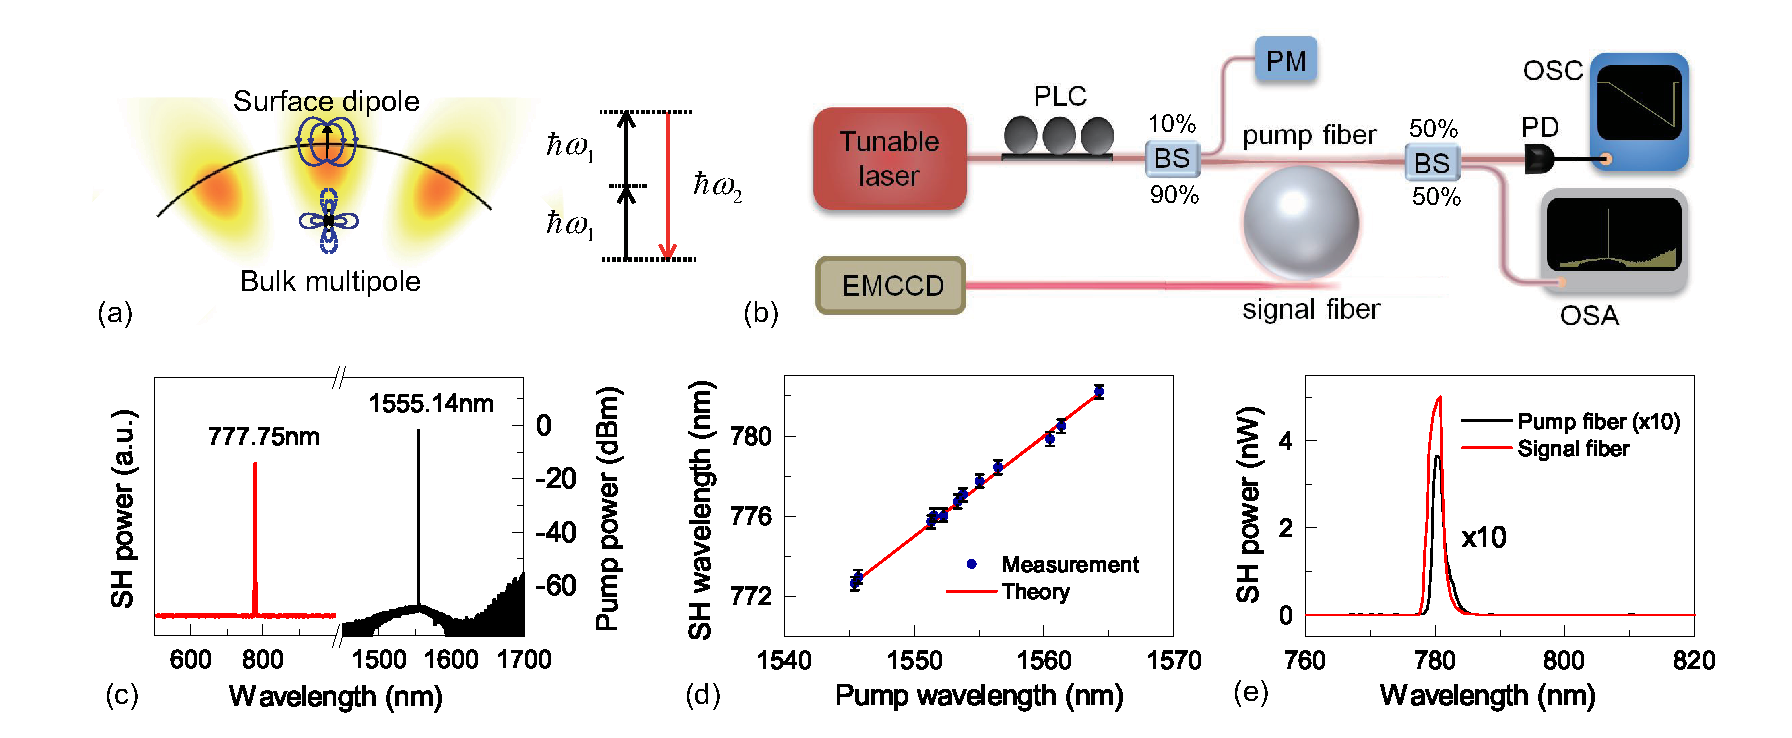
\includegraphics[width=18cm]{Fig1.eps}
\caption{\textbf{Experimental set-up and observation of cavity-enhanced SH signals. a, }The pump light from a tunable laser around 1550 nm is coupled into a silica microsphere through a tapered fiber, and a second fiber is used to collect the SH signal. OSC: oscilloscope. OSA: optical spectrum analyzer. PLC: polarization controller. BS: beam splitter. EMCCD: electron-multiplying CCD. \textbf{b, }SH is generated from the surface dipole response and the bulk multipole response in a WG microsphere. \textbf{c, }Measured SH spectrum (red) and the corresponding pump spectrum (black). \textbf{d, }Measured SH wavelengths versus the corresponding pump wavelengths when different modes are pumped. \textbf{e, }Comparison of SH power collected by signal fiber and pump fiber (10 times magnified).}
\label{pic:Fig1}
\end{figure*}




Here, second harmonic, originating from symmetry breaking at the surface and bulk multipole response (Fig. \ref{pic:Fig1}b), is observed under the continuous wave pump below 1 mW in a WGM microsphere made of centrosymmetric material. 
An unprecedented conversion efficiency of $0.049\%$ W$^{-1}$ benefits from doubly resonant enhancement of ultrahigh $Q$ modes (phase-matching condition[also know as perfect phase matched]), which is achieved by thermal effect and optical Kerr effect. 
% Apart from the compensation of cavity mode dispersion[], Additionally, the collecting efficiency of SH signal is significantly increased with the incorporation of a signal tapered fiber. 
The work enriches the nonlinear toolbox of microcavity photonics and largely extends the emission range of silica microresonators with ultralow pump power, making it possible to push the frequency conversion process down to the quantum regime[refs in Asano OL]. More significantly, the fruitful surface SHG and SFG detection methods can be introduced into (bridged with?) the sensitive microcavity sensing, which enables surface-specific detection with low pump power and high sensitivity.
%The work paves the way for low power and continuous-wave SH sensing. The combination of resonant enhancement and silica surface may enable a series of nonlinear sensitive detection. [BROAD BAND FREQUENCY CONVERSION+SURFACE SENSING]
%\section{Experimental set-up and observation of second harmonic signal}
%[Explain the set-up and how to collect the signal; show the typical spectra and corresponding experimental conditions; explain why other nonlinear processes are absent; f1f2 comparison and conditions]

\begin{figure*}[!ht]
\centering
%\captionsetup{singlelinecheck=no, justification = RaggedRight}
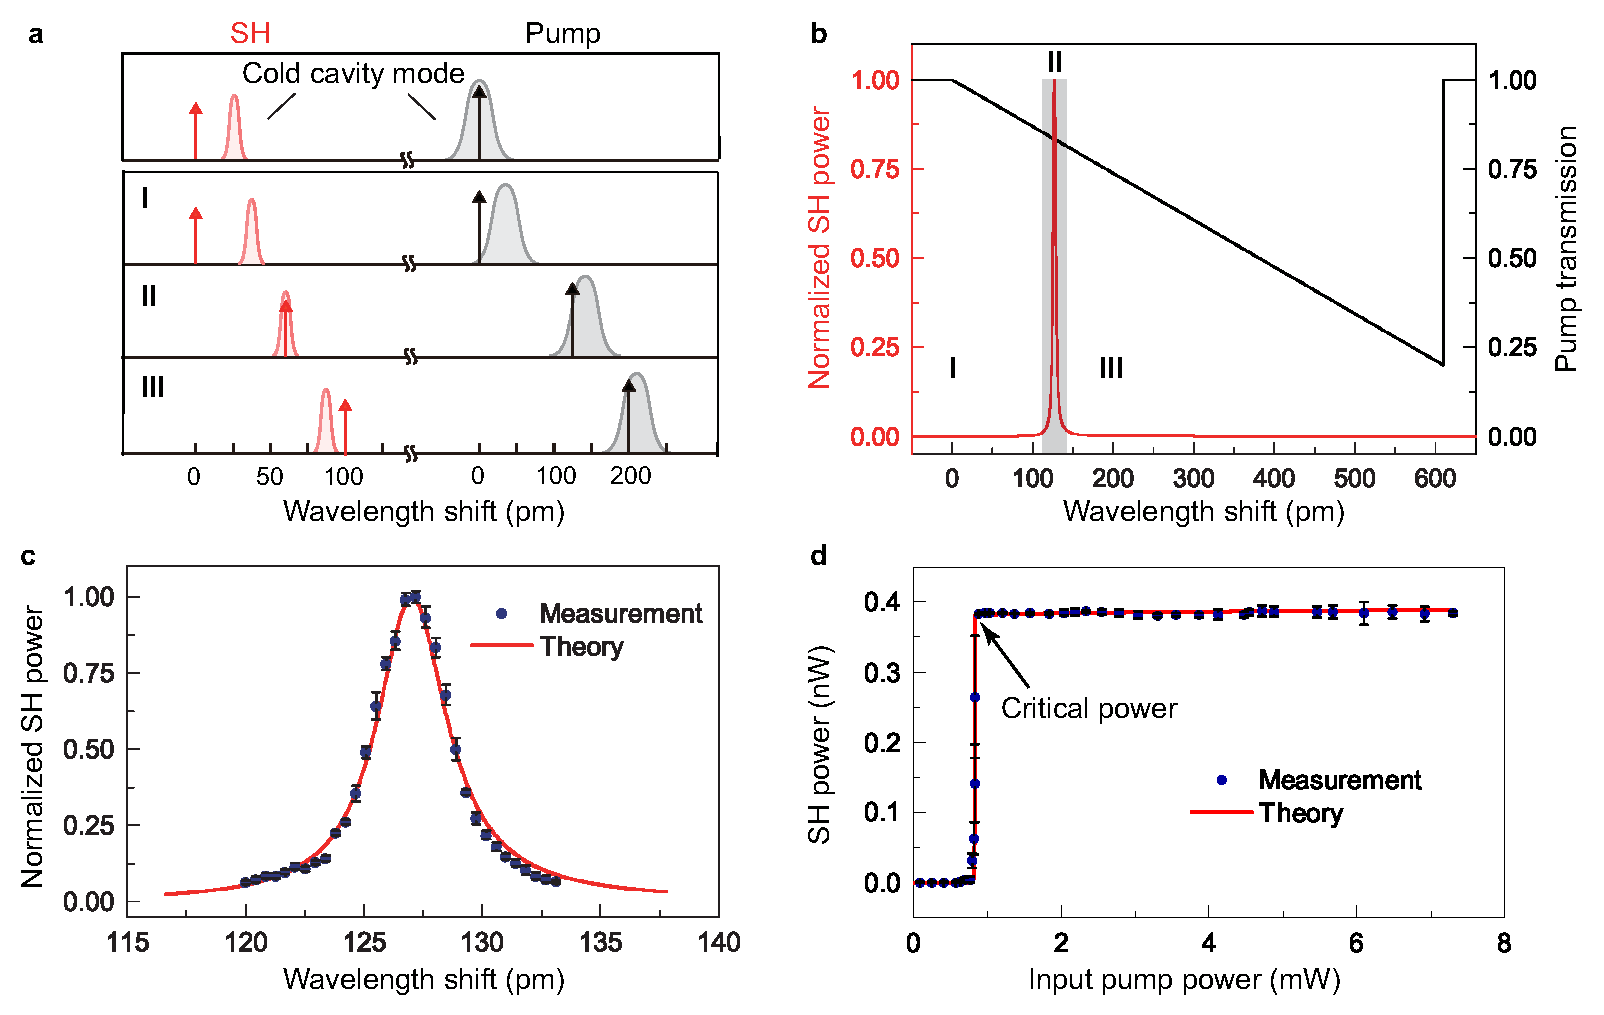
\includegraphics[width=17cm]{try_ed3.eps}
\caption{\textbf{Thermal effect and Kerr effect assisted phase-matching. a, }Schematic of the phase-matching process. Detuning here is the wavelength relative to the cold-cavity wavelength of the pumped mode (to half of this wavelength for SH detuning). The black (red) arrow represents the detuning of the pump light (its SH). The gray (red) Lorentzian line represents the pumped mode (SH mode). 1-3 show three states with increasing pump wavelength but the same input power. \textbf{b, }Normalized SH power and the pump transmission at different pump wavelength detuning. 1-3 correspond to the three states in panel \textbf{a}. The gray area is enlarged in panel \textbf{c} as the theoretical red line. \textbf{c, }SH power versus pump detuning with the input power of 4.46mW. \textbf{d, }The dependence of maximum SH power at all the pump detuning on the input power.}
\label{pic:Fig2}
\end{figure*}

In the experiment, a silica microsphere (diameter $\sim$ $62$ $\upmu$m) 
is pumped through a tapered optical fiber (waist diameter $\sim$ $1$ $\upmu$m) at $1550$ nm band \cite{knight1997phase, cai2000observation}, as shown in Fig. \ref{pic:Fig1}a. To collect SH signal efficiently, a second fiber taper (waist diameter $\sim$ 0.5 $\upmu$m) designed for 780 nm band is incorporated into the system. The intrinsic quality factor (Q) for the pumped cavity mode is $4.8\times10^7$. %When the signal tapered fiber is near the microsphere to couple SH signals, the effective intrinsic Q (including the intrinsic loss and loss induced by the signal fiber) decreases and a typical value is $3.6\times 10^7$.%The signals collected by the signal tapered fiber are sent into an electron-multiplying CCD (EMCCD) to extract the spectra.
% The EMCCD and the pump laser are placed at the same side of the microsphere considering the linear momentum conservation requirement in SHG\cite{carmon2007visible, kozyreff2008whispering}.
% A tapered fiber phase-matched at the telecommunication band couples the pump into the microsphere. This tapered fiber is not able to collect the second harmonic signal efficiently due to phase mismatch at around 780 nm and the high radial order of the second harmonic mode\cite{carmon2007visible}. To overcome this problem and collect weak second harmonic signals, another tapered fiber (signal tapered fiber) designed to achieve phase matching condition at second harmonic wavelength is fabricated together with the pump tapered fiber and incorporated into the system as is shown in Fig.\ref{pic:Fig1}a. The tapered fibers can reach critical coupling simultaneously at around 1555 nm and 777 nm. 
% A fiber coupler split 10\% of the pump power from the laser into a power meter to monitor the input power. 
Figure \ref{pic:Fig1}\textbf{c} shows a typical SH spectrum measured from the electron-multiplying CCD (EMCCD) and the corresponding pump spectrum measured from the optical spectrum analyzer (OSA). The SH signal appears at $777.75$ nm when pumped at $1555.14$ nm, which deviates only $0.023$\% from the expected wavelength, falling into the resolution tolerance of OSA and EMCCD.
Note that stimulated Raman scattering and parametric oscillation do not occur because their thresholds are far above the pump power in the experiment. % \cite{spillane2002ultralow, kippenberg2004kerr}. 
Third harmonic generation is also absent due to the phase mismatch in the nonlinear optical process.
% between the mode and its third harmonic modes\cite{carmon2007visible}. 
%Third harmonic signals  collected by the signal fiber are also observable when pumped at some specific modes [need figure?]. 
%[e, ->d]
Moreover, SH signals arise in the full range when cavity modes are pumped from $1545$ nm to $1565$ nm, as shown in Fig. \ref{pic:Fig1}d.
%Thanks to the plethora of modes in the microsphere, SH signals arise in , which is 
Among the occurrence of SH, a maximum signal power of $5$ nW was observed via the signal fiber. To compare the collecting efficiency of the two fibers, we optimize the fiber-cavity coupling so that the SH signal from the pump fiber is also observable, but the maximum signal power is still over one order of magnitude weaker than that from the signal fiber. From either fibers, SH signal is absent when the pump is off-resonance with cavity modes, which helps to eliminate the possibility of spurious signals such as the second order diffraction of the EMCCD grating.
%Using the signal fiber, an SH signal with a power of  (shown in Fig.\ref{pic:Fig1}c) is collected at the pump wavelength of 1561.3 nm. 
%The SH power is calibrated from the EMCCD spectra to represent the power in the signal fiber near the microsphere. 
%In order to compare the collecting efficiency, the pump tapered fiber is connected directly to the EMCCD and the coupling between the pump fiber and the microsphere is optimized to maximize the collected SH power. The SH signal is still observable but the maximum power is only 0.36 nW, which is more than 13 times weaker than the SH power collected by the signal fiber.

%The SH signal is only present when the pump light is in the mode (judging from the transmission). Because of thermal bistability\cite{carmon2004dynamical}, the pump light can be out of the mode when tuning the wavelength to blue side but in the mode when tuning in the opposite direction. At the same wavelength, only the in-mode pump can produce the SH. And the SH signal is always absent when the microsphere is moved far from the pump fiber, which also help to eliminate the possibility of spurious signals created by the second order diffraction of the EMCCD grating.



%The signal tapered fiber in this set-up is critical to collect SH signals efficiently. 


%\section{Thermal effect and Kerr effect assisted phase-matching}
%[Prerequisite phase matching (higher order radial modes) and its problems; P2-P1 relation and how to enhance SH signals; mechanisms for assisted phase-matching; results: dependence on detuning and power; comparison with other SH and silica sphere TH.]

% The enhancement of SH power by ultrahigh-Q microresonator is obvious in eq.(\ref{eq:P2P1}). 

The doubly resonant enhancement plays a pivotal role in efficient SHG, which is achieved by perfect phase-matching including momentum conservation and energy conservation.
%, lies in the heart of  and reaching the high conversion efficiency. 
%The ultrahigh Q represents the factor of enhancement but also presents a challenge to phase matching or double resonance in a microresonator\cite{carmon2007visible, kozyreff2008whispering, xu2008second, farnesi2014optical}($\omega_p = \omega_1, 2\omega_p = \omega_2$). 
The former can be fulfilled by a pair of modes with proper angular momentum relation $m_2=2m_1$, where $m_1$ ($m_2$) is the angular number of the pump (SH) cavity mode. 
However, the material and geometric dispersion presents a challenge on energy conservation, obstructing the double resonance $\omega_2=2\omega_1$ and consequently, efficient SHG. 
%The dependence of SH power on pump power can be derived from .
More accurately, the SH power can be derived from coupled mode equations (see Supplementary Information)%\cite{haus1991coupled}
\begin{equation}
P_2 = \frac{4|g|^2Q_2^2/(\omega_2Q_{1e})}{4Q_2^2(2\omega_p/\omega_2-1)^2+1}\frac{16Q_1^4P_1^2/(\omega_1Q_{2e})^2}{[4Q_1^2(\omega_p/\omega_1-1)^2+1]^2},
\label{eq:P2P1}
\end{equation}
where the subscripts 1, 2 represent the pumped mode and SH mode respectively, $\omega_i$ is the mode frequency and $\omega_p$ is the pump frequency, $P_1$ denotes the input pump power, $g$ is the coupling coefficient between two modes, %, which will be looked into in the next section. 
$Q_i$ ($i=1, 2$) stands for the loaded quality factor %$\eta_{i}=Q_i/Q_{ie}$ is the coupling factor 
and $Q_{ie}$ represents the external quality factor. The pump power depletion is ignored due to the weak second order nonlinear effect in silica.
Equation (\ref{eq:P2P1}) shows that ultrahigh $Q$ is indispensable in boosting the SH power, while it also presents a challenge in double resonance by magnifying the frequency mismatch induced by the material and geometric dispersion.
%, which manifests the significance of double resonance ($\omega_1 = \omega_p = \omega_2/2$).
In order to compensate the dispersion, SH modes with higher order radial number was proposed or used  \cite{kozyreff2008whispering}[other], which relies on delicate geometric design of the cavity.
%For SHG, a silica microsphere with a diameter of $60$ $\upmu$m gives rise to good phase-matching between a fundamental mode near $1550$ nm and an SH mode with radial number $q_2=2$ (see Supplementary Information). 
In the experiment, however, the desired phase-matching can be disturbed by the deviation of cavity from its designed geometry, making one of the mode off-resonance and impeding highly efficient SHG. 
%But due to the discrete distribution of modes, the mode with smallest phase mismatch can reduce the SH power by a factor of $10^{-6}$. This phase matching method is also extremely sensitive to the size of microresonators. A deviation of 3\% in diameter can lead to a reduction of SH power by nearly 4 orders of magnitude. It is difficult to control the size of a microsphere precisely in the experiments. 
Therefore, to tune the cavity dispersion precisely and dynamically, we propose and experimentally realize a versatile method, leveraging mode frequency shift induced by thermal behavior (namely thermal expansion, thermally induced refractive index change and the optical Kerr effect) \cite{del2011octave, herr2014temporal}.
%Thermal effect and Kerr effect have been utilized to compensate the dispersion in microresonator-based frequency comb generation. These effects can also help to achieve phase matching in SHG. 
%Both of the two effects lead to a red shift of the mode frequency \cite{ilchenko1992thermal, treussart1998evidence,  carmon2004dynamical, fomin2005nonstationary} and there is no need to distinguish them because the focus is steady state continuous wave emission. [NEED IT OR NOT?]

The mechanism of thermal and Kerr assisted phase matching process is illustrated in Fig. \ref{pic:Fig2}a. 
When the pump power is weak and the mode frequency shift is negligible (cold cavity), the pumped ($\omega_{10}$) and SH modes ($\omega_{20}$) usually cannot be on resonance with the pump light and its SH simultaneously. 
With a larger input power, the pump mode experiences a red shift due to xxx: $\omega_1 = \omega_{10}-B_{11}|\alpha_1|^2$, where $|\alpha_1|^2$ is the intra-cavity power of the pumped mode and $B_{11}$ is the coefficient of pump frequency shift. In this case, the wavelength of pump light should also increase to catch the pump mode, resulting in the non-Lorentzian, triangular transmission shape [carmon2004].
The SH mode also exhibits a red shift from the cold cavity frequency, which can be described by $\omega_2 = \omega_{20}-B_{12}|\alpha_1|^2$ where $B_{12}$ is the coefficient of SH frequency shift. The thermal and Kerr effects of the SH are ignored in the analysis.
In the process of tuning pump frequency from the cold cavity mode to resonance with the pump mode (state 1-3 in Fig. \ref{pic:Fig2}a), the larger rate of red shift for the SH of pump light ($\omega_p/2$) helps it to catch the SH mode ($\omega_2$) at a certain pump-cavity detuning  where the phase-matching condition is fulfilled the SH power reaches a peak value (state 2).
Because of the ultrahigh $Q$ of the SH resonance, the SH power diminishes rapidly before and after reaching the on-resonance frequency for SH (state 1 and 3 in Figs. \ref{pic:Fig2}a and b). 
xxx phase matching can also be realized in other cases with different rate of SH mode frequency shift or initial detuning between $\omega_p/2$ and $\omega_2$ (see SI).

%At the on-resonance pump frequency for SH, the phase-matching condition is fulfilled and the SH power reaches a peak value (corresponding to state 2 in fig.\ref{pic:Fig2}a and b). 


Using the phase matching method, we measure the SH power by tuning the pump frequency in the range of the gray area (Fig. \ref{pic:Fig2}b) with a fixed input power, as shown in Fig. \ref{pic:Fig2}c.%  is measured % of $4.46$ mW. [fitting results here]
Furthermore, the dependence of SH power on pump power is studied, as presented in Fig. \ref{pic:Fig2}d. 
Under each input power, we search for the maximum SH output power in the detuning range from the cold cavity mode to the on-resonance frequency for the pump. 
Among different values of input power, a critical power manifests itself, at which the SH of pump light achieves the resonance condition exactly when the pump becomes exactly resonant. % and its SH achieve double resonance simultaneously,% the  power arrives at the peak value just before the pump light becomes on resonance.% and then thermally unlocked. 
In this case, the SH power is able to arrives at the peak value in Fig. \ref{pic:Fig2}c, which represents the most efficient SHG with the pump power of $879$ $\upmu$W and the conversion efficiency of $0.049\%$ W$^{-1}$.
Below the critical power, the SH of pump light is off resonance within the full detuning range, resulting in the extremely weak SH power.
Above the critical power, the increasing input power at a fixed frequency pushes the pump mode farther to the red side (the pump is not completely on resonance) and consequently increases the detuning between the pump light and the cavity.
The resulting reduced enhancement of the pump light counteracts with the increasing input power, leading to the almost steady intracavity power. [SI]
The on-resonance frequency of the SH mode also remains unchanged with increasing input power, so that the intracavity power and consequently the SH power are almost unchanged as well. % is determined by the intracavity power and the pump frequency, that is, $2\omega_p = \omega_2(|\alpha_1|^2)$.
%Consequently, the SH power remains the same with increasing input power.


%[The red shift of the SH mode is proportional to the intra-cavity power, which is proportional to the pump light detuning from the cold cavity frequency. It means $\Delta \omega_2 = D_{12}\Delta \omega_p$, where $\Delta \omega_2$ is the SH mode frequency shift, $\Delta \omega_p$ is the pump light detuning and $D_{12}$ is the proportionality coefficient.  Using this relation and eq.(\ref{eq:P2P1}), the experimental parameters can be fit by the theory to be $Q_2\times(2-D_{12})=8.57\times 10^5$.]
%[Fitting]
%The critical input power is fitted to be 832.5$\upmu$W and the corresponding SH power is fitted to be 381pW. 
%Eq.(\ref{eq:P2P1}) and $\omega_1 = \omega_{10}-B_{11}|\alpha_1|^2$ \cite{carmon2004dynamical}, $\omega_2 = \omega_{20}-B_{12}|\alpha_1|^2$ are used to fit the experimental data, where $\omega_{i0}$ is the mode frequency in the cold cavity, $|\alpha_1|^2$ is normalized to the intra-cavity power of the pumped mode and $B_{1i}$ is the coefficient of intra-cavity power induced frequency shift. The parameters related to the pumped mode can be extracted from the measurements. 
%Increasing the input power leads to the appearance and broadening of the  for the pump\cite{carmon2004dynamical}, resulting from the mo 
%When the pump power is large enough, the pumped mode shifts more to the red side with increasing intra-cavity power. Tuning the pump frequency from the cold cavity mode to the red side can decrease the detuning $\omega_p-\omega_1$ and increase intra-cavity power, thus making the triangular resonance shape \cite{carmon2004dynamical}. 





%When the mode in Fig.\ref{pic:Fig1}b is pumped with an input power of 4.46 mW, the SH power exhibits a clear peak at the pump wavelength of 1555.14 nm, which is shown in fig.\ref{pic:Fig2}c. 


% [EXPLANATION OF WHY THE INTRACAVITY POWER REMAIN ALMOST UNCHANGED]
%The thermal and Kerr assisted phase matching makes the SH power depend strongly on the pump frequency, which also determines the intra-cavity pump power. At a certain pump frequency (the mode frequency is still at the red side of the pump), when the input power increases, the intra-cavity power also tends to increase, which pushes the mode frequency to the redder side. The pump frequency remains unchanged so that the detuning $\omega_p-\omega_1$ increases to lower the coupling efficiency of the input power into the cavity. Therefore, the intra-cavity pump power increases more slowly than the increase of input pump power. 


%The dependence of SH power and intra-cavity power on the pump frequency gives rise to a novel relation between the SH power ($P_2$) and the input pump power ($P_1$). When $P_1$ is not large enough for the pump SH to catch the SH mode before the pump frequency catches the mode frequency, the SH mode cannot be on resonance at any pump frequency and the SH power is small because of the ultrahigh Q. When $P_1$ reaches a critical power so that the pump SH and the pump frequency catch the two modes simultaneously, the two denominators in eq.(\ref{eq:P2P1}) reach the smallest value of 1, which gives rise to an efficient SHG. When $P_1$ further increases from the critical power, the intra-cavity power increases slowly so that the SH-on-resonance frequency also moves slowly, therefore, when the pump SH is on resonance with the SH mode, the intra-cavity pump power and the corresponding SH power does not change as rapidly as the input pump power.  



\begin{figure*}[!ht]
%\centering
%\captionsetup{singlelinecheck=no, justification = RaggedRight}
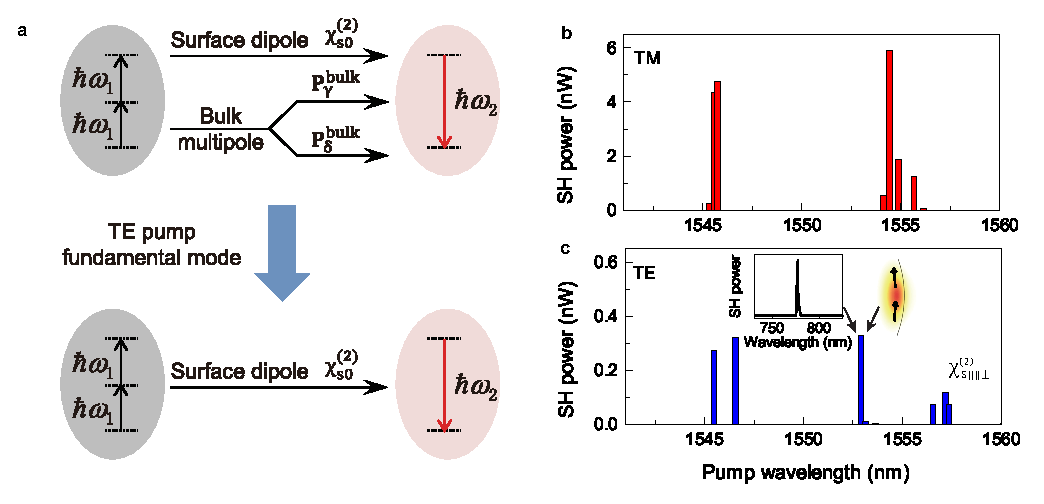
\includegraphics[width=18cm]{Fig3new.eps}
\caption{\textbf{Identification of surface nonlinearity from the bulk multipole response. a, }Origin of second order nonlinearity and the method to obtain surface-only nonlinear coupling. \textbf{b,c,} Measured second harmonic power at the corresponding pump wavelength with TM (\textbf{b}) and TE (\textbf{c}) pump polarization respectively. Inset in \textbf{c}: Field distribution of the target mode from numerical simulation(left) and measurement (right).}
\label{pic:Fig3}
\end{figure*}

%[where?]
%In the THG experiments in silica microresonators\cite{carmon2007visible, farnesi2014optical}, the phase mismatch curve is flat for high order radial modes, and the shift speed of the pump TH frequency and the TH frequency mode may be similar. Consequently, the high order radial modes induced phase matching may play a major role so that the $P_1^3$ relation can be observed. 
Microresonator SHG in other materials usually use different phase matching strategy to achieve broadband phase matching, e.g. quasi-phase-matching [cite more later]. The quality factor is also moderate so that the thermal effect and Kerr effect do not manifest themselves in the SHG process. 
With xxx phase matching, it is also possible to obtain the explicit $P_2 \propto P_1^2$ dependence by introducing a degree of freedom other than the pump intracavity power to manipulate the SH mode frequency. 
For example, a control light or a heater can be incorporated into the system to change the intra-cavity power and thus achieving the double on-resonance condition at various input pump power. 
The specific measurement plan is beyond the scope of this [letter?].% and is still under investigation.


%\section{Origin of second order nonlinearity}



%[Theory for surface \& bulk 2nd nonlinearity; relationship with polarization]

%Silica is a centrosymmetric material in which the electric dipole induced second order nonlinearity is forbidden (see \cite{boyd2003nonlinear} for reference). Surface symmetry broken and bulk multipole become the major sources of second order nonlinearity (see \cite{heinz1991second} for review). 

%Apart from the unique power response, the SH power enhanced by the microresonator also exhibits a polarization dependence. 
%In the experiment, transverse magnetic (TM) or transverse electric (TE) modes from $1545$ nm to $1565$ nm are pumped separately by adjusting the polarization of the pump light. 
%The maximum SH power of each SHG process is recorded for the two polarization respectively, as shown in the histogram in Fig. \ref{pic:Fig3}. 
%After traversing the wavelength range with each polarization, a total number of $69$ ($40$) SHG incidence is recorded for TM (TE) polarization, and the average SH power is $0.843$ nW ($0.619$ nW). 
In order to distinguish the contributions of surface and bulk nonlinearity, we investigate the polarization dependence, which originates from the % polarization dependent 
nonlinear coupling strength $g$ in equation (\ref{eq:P2P1}). %, which can be derived from the Helmholtz equation and the relation between electric field and nonlinear polarization. %, which bridges the microresonator with the second order nonlinearity of centrosymmetric material. 
%Using , the coupling coefficient induced by 
%The second order nonlinear coupling arises from the breaking inversion symmetry at the surface and the bulk multipole response.
The nonlinear coupling strength from surface dipole response can be written as
\begin{equation}
g_{s0} = 2\frac{\omega_1^2}{\omega_2n^2}\frac{\int_{\mathrm{surface} } \mathbf{E}_{02}^*:\upchi^{(2)}_{s0}:\mathbf{E}_{01}\mathbf{E}_{01} \mathrm{d}	\mathbf{S}}{\int |\mathbf{E}_{02}|^2 \mathrm{d}	\mathbf{V}}
\end{equation}
where $n$ is the refractive index, $\upchi^{(2)}_{s0}$ represents the surface nonlinear susceptibility, and $\mathbf{E}_{0i}(\mathbf{x})$ denotes the  normalized electric field. % so that $\alpha_i\mathbf{E}_{0i}(\mathbf{x})$ is the complete electric field. 
The bulk multipole nonlinear polarization in silica can be expressed as $\mathbf{P}^{\mathrm{bulk}} =  \gamma\nabla(\mathbf{E}\cdot\mathbf{E})+\delta(\mathbf{E}\cdot\nabla)\mathbf{E}$ [ref], where $\gamma$ and $\delta$ are the nonlinear coefficients. The first term $\mathbf{P}^{\mathrm{bulk}}_\gamma$ represents a longitudinal wave which can excite SH only at the surface. Therefore $\mathbf{P}^{\mathrm{bulk}}_\gamma$ can contribute to an effective surface susceptibility $\upchi^{(2)}_s = \upchi^{(2)}_{s0}+\upchi^{(2)}_{s,\gamma}$\cite{heinz1991second}, corresponding to an effective coupling strength of $g_s$. The coupling strength induced by the second term $\mathbf{P}^{\mathrm{bulk}}_\delta$ can be written as % $a'$
\begin{equation}
g_b =  2\frac{\omega_1^2}{\omega_2n^2}\frac{\delta \int \mathbf{E}_{02}^* \cdot (\mathbf{E}_{01}\cdot\nabla)\mathbf{E}_{01} \mathrm{d}	\mathbf{V}}{\int |\mathbf{E}_{02}|^2 \mathrm{d} \mathbf{V}}
\label{eq:gb}
\end{equation}
Thus the total second order nonlinear coupling strength $g = g_s+g_b$, as shown in Fig. \ref{pic:Fig3}a.

The effective surface susceptibility tensor $\upchi^{(2)}_s$ contains three non-zero components $\upchi_{\perp \perp \perp}$, $\upchi_{\parallel \parallel \perp}$ and $\upchi_{\perp \parallel \parallel}$, where $\perp$ denotes the electric field direction perpendicular to the surface and $\parallel$ corresponds to the parallel direction. 
$\upchi_{\perp \parallel \parallel}$ can be ignored in studying SHG due to the non-degeneracy of TM and TE pump modes.  
$\upchi_{\perp \perp \perp}$ ($\upchi_{\parallel \parallel \perp}$) plays a major role when TM (TE) mode is pumped, which only generates the TM polarized second harmonic in both cases. 
TM modes are preferable in surface induced SHG because $\upchi_{\perp \perp \perp}$ is larger than $\upchi_{\parallel \parallel \perp}$ \cite{rodriguez2008calibration}. 
Considering the bulk nonlinear response induced by $\mathbf{P}^{\mathrm{bulk}}_\delta$, the coupling strength $g_b$ relies on the specific field distribution in the cavity and the generated SH exhibits the same polarization as the pump mode. 
Note that for TE polarization, the field direction is along the polar direction, so that the polar symmetry of modes prohibits the excitation of SH modes with an even polar distribution from $\mathbf{P}^{\mathrm{bulk}}_\delta$. 
While the TM pump modes, with electric field along the radial direction, can excite second harmonic without the above restriction.
 %the coupling strength $g_b$ involving an SH mode with  for a TE mode, the divergence is along the polar direction, which exhibits geometric symmetry with regard to the equatorial plane. 
%If both the pumped mode and the SH mode are fundamental in the polar direction (polar number $l$ = azimuthal number $m$), $g_b$ vanishes due to the divergence and the polar symmetry. 
Because of a stronger confinement in the radial direction than the polar direction and thus a larger divergence for most of the modes, TM modes tend to link with a larger $g_b$ than TE modes. 
Consequently, from both the surface and the bulk second order nonlinearity, TM pump modes can generate stronger SH signals statistically
In the experiment, transverse magnetic (TM) or transverse electric (TE) modes from $1545$ nm to $1565$ nm are pumped separately by adjusting the polarization of the pump light.
The TM pump modes exhibit larger SH power, as shown in Fig. \ref{pic:Fig3}b and c, which agrees with the theoretical analysis.

%For example, in a silica microsphere with a diameter of 62$\upmu$m, the TM pumped mode with $l_1=m_1=171$ and its SH mode with $l_2=m_2=342$ produces a $g_b$ 18 times larger than that of the TE mode with $l_1-1=m_1=171$ and its SH mode with $l_2-1=m_2=342$ (in both cases, the radial numbers of the pumped mode and SH mode are 1 and 2 respectively due to phase matching considerations). 

The polarization dependence can be utilized to identify the surface nonlinearity from the bulk nonlinear response of both $\mathbf{P}^{\mathrm{bulk}}_\gamma$ and $\mathbf{P}^{\mathrm{bulk}}_\delta$.  %should be eliminated.
The former effect does not contribute to susceptibility $\upchi_{\parallel \parallel \perp}$, corresponding to the TE polarized pump [heinz]. 
% , 
The latter can also be discerned from the surface nonlinear response with the TE polarized pump.
In this case, an SH signal with a TM polarization can only originate from the surface nonlinearity ($\upchi_{\parallel \parallel \perp}$) because $\mathbf{P}^{\mathrm{bulk}}_\delta$ requires the same polarization between the pump mode and the SH mode.
Furthermore, when a fundamental [] TE mode (angular number $l_1=m_1$) is pumped, only the fundamental SH modes (angular number$l_2=m_2$) are allowed by the selection rule [], which cannot be excited from $\mathbf{P}^{\mathrm{bulk}}_\delta$ due to even polar field distribution of the SH mode. 
In the measurement, a surface-only second harmonic is obtained deterministically by employ a fundamental TE pump mode at xx nm without measuring the SH polarization, as shown in the left inset in Fig. \ref{pic:Fig3}c.
Here the fundamental TE pump mode is confirmed experimentally by measuring the transmission while scanning the relative angular position of the pump fiber and the cavity, as illustrated in the  Fig. \ref{pic:Fig3}c.
%In order to select a TE pump mode, 
%  and obtain  .

%Mediated by , two TE polarized photons can generate a TM polarized photon. For nonlinearity from bulk multipole effects ($g_b$), TE polarized pump can only generate TE SH. In this case, the bulk response can be eliminated and thus restricting the SHG on the surface.



\begin{figure}[!ht]
\centering
%\captionsetup{singlelinecheck=no, justification = RaggedRight}
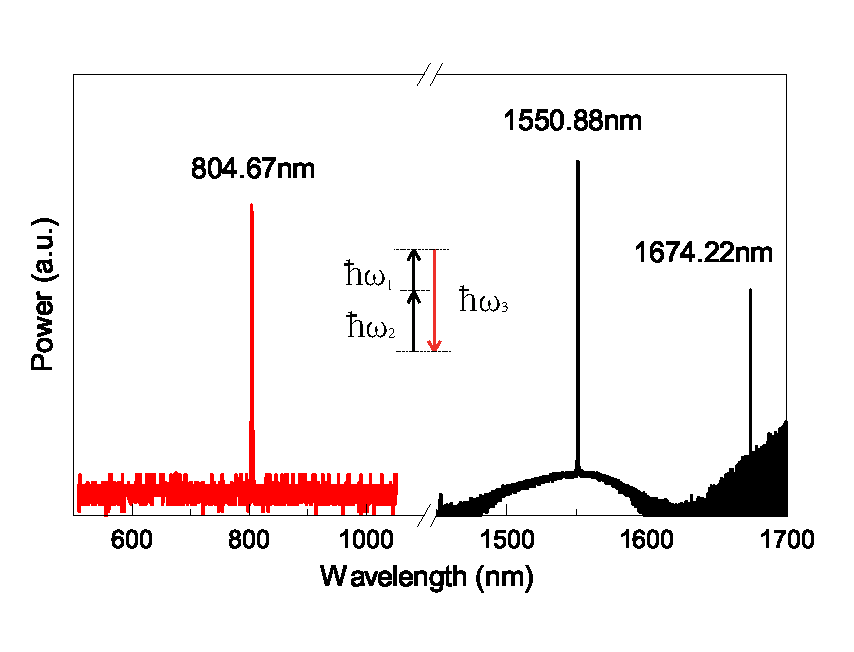
\includegraphics[width=8cm]{Fig4.eps}
\caption{\textbf{Measured spectra of second-order sum frequency generation (SFG). }The pump light ($\omega_1$) and Raman light ($\omega_2$) are summed to generate the SF signal ($\omega_3$).}
\label{pic:Fig4}
\end{figure}


%[More eg of SH; sum frequency]

Additionally, sum frequency generation (SFG) can also arise when a Raman signal is stimulated by the pump light. 
Shown in Fig. \ref{pic:Fig4} is an SF signal ($804.67$ nm) and the corresponding pump ($1550.88$ nm) and its Raman signal ($1674.22$ nm) with an input power of $7.33$ mW, which is above the Raman threshold for this mode. 
The deviation of the SF wavelength from the expected value ($804.63$ nm) is much smaller than the resolution of EMCCD.
%The measured wavelengths satisfy the SFG relation $1/1550.88$ $\mathrm{nm} +1/1674.22$ $\mathrm{nm} = 1/804.63$ $\mathrm{nm}$, which is close to the measured SF wavelength 804.67 nm.

%[Conclusion]
For the first time, to the best of our knowledge, the second harmonic from breaking of inversion symmetry at the surface  is deterministically observed in a silica microresonator without the influence of bulk multipoles. 
This work opens up a new direction to focus on the surface nonlinearity with double resonance enhancement, where the detectable SH signal under submilliwatt pump power demonstrates the potential of studying surface properties and detecting molecules with ultrahigh sensitivity. 
The ultralow operating power, compactness of the device and simplicity of measurement also enables a novel label-free biological molecule sensing, which can potentially be integrated. 
Additionally, the phase-matching method we used does not rely on the specific geometry and material of the cavity, making it possible to extend the surface SHG into other microcavity systems such as microtoroid, microdisk and microring with different centrosymmetric materials.
The possibility of SHG in different microresonators may also give rise to second-harmonic-assisted phenomena in frequency comb generation.
In quantum optics applications, this work also represents a remarkable step towards the second order nonlinearity mediated squeezing and entangled pair generation.
 




\bibliography{ref}
\end{document}

